\documentclass[1p]{elsarticle_modified}
%\bibliographystyle{elsarticle-num}

%\usepackage[colorlinks]{hyperref}
%\usepackage{abbrmath_seonhwa} %\Abb, \Ascr, \Acal ,\Abf, \Afrak
\usepackage{amsfonts}
\usepackage{amssymb}
\usepackage{amsmath}
\usepackage{amsthm}
\usepackage{scalefnt}
\usepackage{amsbsy}
\usepackage{kotex}
\usepackage{caption}
\usepackage{subfig}
\usepackage{color}
\usepackage{graphicx}
\usepackage{xcolor} %% white, black, red, green, blue, cyan, magenta, yellow
\usepackage{float}
\usepackage{setspace}
\usepackage{hyperref}

\usepackage{tikz}
\usetikzlibrary{arrows}

\usepackage{multirow}
\usepackage{array} % fixed length table
\usepackage{hhline}

%%%%%%%%%%%%%%%%%%%%%
\makeatletter
\renewcommand*\env@matrix[1][\arraystretch]{%
	\edef\arraystretch{#1}%
	\hskip -\arraycolsep
	\let\@ifnextchar\new@ifnextchar
	\array{*\c@MaxMatrixCols c}}
\makeatother %https://tex.stackexchange.com/questions/14071/how-can-i-increase-the-line-spacing-in-a-matrix
%%%%%%%%%%%%%%%

\usepackage[normalem]{ulem}

\newcommand{\msout}[1]{\ifmmode\text{\sout{\ensuremath{#1}}}\else\sout{#1}\fi}
%SOURCE: \msout is \stkout macro in https://tex.stackexchange.com/questions/20609/strikeout-in-math-mode

\newcommand{\cancel}[1]{
	\ifmmode
	{\color{red}\msout{#1}}
	\else
	{\color{red}\sout{#1}}
	\fi
}

\newcommand{\add}[1]{
	{\color{blue}\uwave{#1}}
}

\newcommand{\replace}[2]{
	\ifmmode
	{\color{red}\msout{#1}}{\color{blue}\uwave{#2}}
	\else
	{\color{red}\sout{#1}}{\color{blue}\uwave{#2}}
	\fi
}

\newcommand{\Sol}{\mathcal{S}} %segment
\newcommand{\D}{D} %diagram
\newcommand{\A}{\mathcal{A}} %arc


%%%%%%%%%%%%%%%%%%%%%%%%%%%%%5 test

\def\sl{\operatorname{\textup{SL}}(2,\Cbb)}
\def\psl{\operatorname{\textup{PSL}}(2,\Cbb)}
\def\quan{\mkern 1mu \triangleright \mkern 1mu}

\theoremstyle{definition}
\newtheorem{thm}{Theorem}[section]
\newtheorem{prop}[thm]{Proposition}
\newtheorem{lem}[thm]{Lemma}
\newtheorem{ques}[thm]{Question}
\newtheorem{cor}[thm]{Corollary}
\newtheorem{defn}[thm]{Definition}
\newtheorem{exam}[thm]{Example}
\newtheorem{rmk}[thm]{Remark}
\newtheorem{alg}[thm]{Algorithm}

\newcommand{\I}{\sqrt{-1}}
\begin{document}

%\begin{frontmatter}
%
%\title{Boundary parabolic representations of knots up to 8 crossings}
%
%%% Group authors per affiliation:
%\author{Yunhi Cho} 
%\address{Department of Mathematics, University of Seoul, Seoul, Korea}
%\ead{yhcho@uos.ac.kr}
%
%
%\author{Seonhwa Kim} %\fnref{s_kim}}
%\address{Center for Geometry and Physics, Institute for Basic Science, Pohang, 37673, Korea}
%\ead{ryeona17@ibs.re.kr}
%
%\author{Hyuk Kim}
%\address{Department of Mathematical Sciences, Seoul National University, Seoul 08826, Korea}
%\ead{hyukkim@snu.ac.kr}
%
%\author{Seokbeom Yoon}
%\address{Department of Mathematical Sciences, Seoul National University, Seoul, 08826,  Korea}
%\ead{sbyoon15@snu.ac.kr}
%
%\begin{abstract}
%We find all boundary parabolic representation of knots up to 8 crossings.
%
%\end{abstract}
%\begin{keyword}
%    \MSC[2010] 57M25 
%\end{keyword}
%
%\end{frontmatter}

%\linenumbers
%\tableofcontents
%
\newcommand\colored[1]{\textcolor{white}{\rule[-0.35ex]{0.8em}{1.4ex}}\kern-0.8em\color{red} #1}%
%\newcommand\colored[1]{\textcolor{white}{ #1}\kern-2.17ex	\textcolor{white}{ #1}\kern-1.81ex	\textcolor{white}{ #1}\kern-2.15ex\color{red}#1	}

{\Large $\underline{12n_{0270}~(K12n_{0270})}$}

\setlength{\tabcolsep}{10pt}
\renewcommand{\arraystretch}{1.6}
\vspace{1cm}\begin{tabular}{m{100pt}>{\centering\arraybackslash}m{274pt}}
\multirow{5}{120pt}{
	\centering
	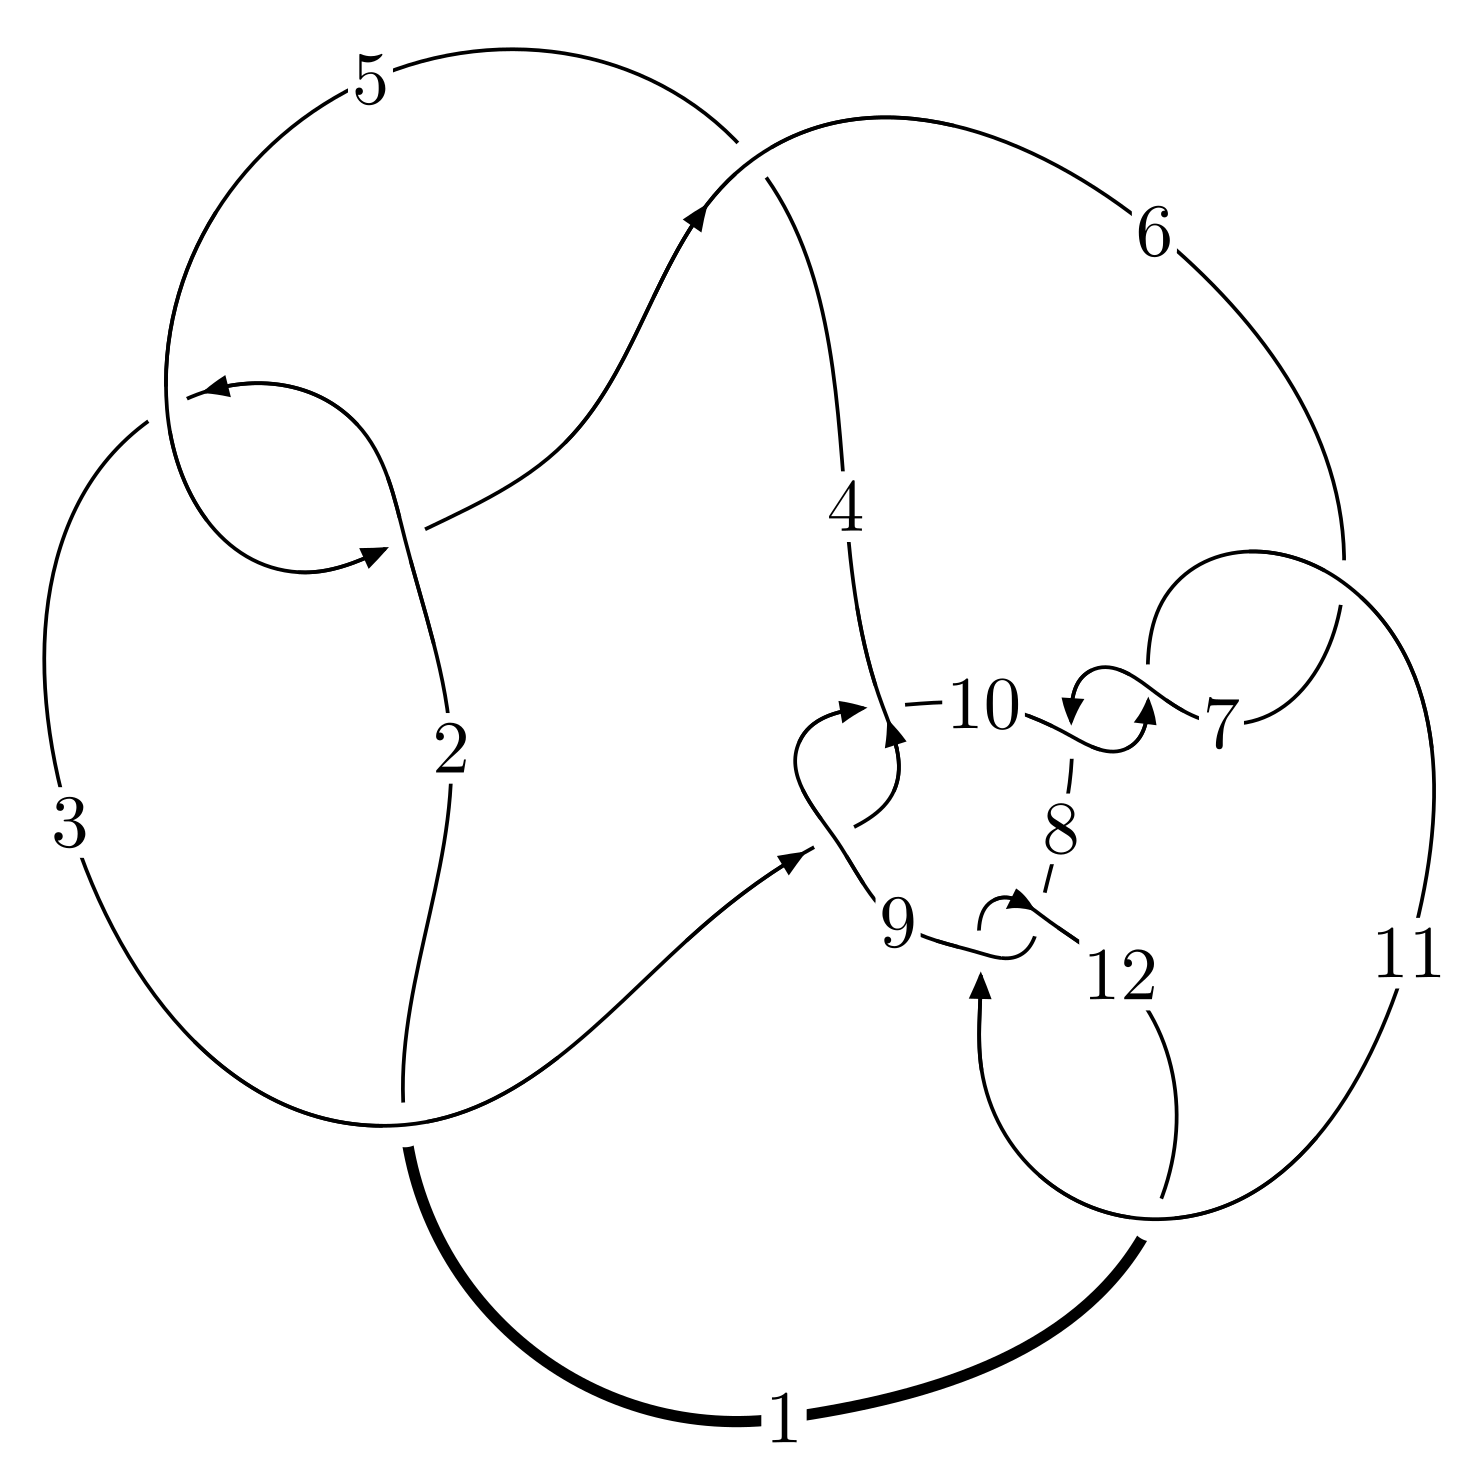
\includegraphics[width=112pt]{../../../GIT/diagram.site/Diagrams/png/2359_12n_0270.png}\\
\ \ \ A knot diagram\footnotemark}&
\allowdisplaybreaks
\textbf{Linearized knot diagam} \\
\cline{2-2}
 &
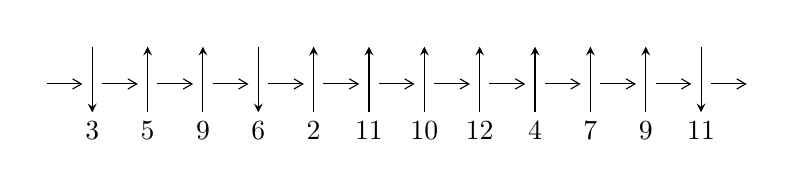
\begin{tikzpicture}[x=20pt, y=17pt]
	% nodes
	\node (C0) at (0, 0) {};
	\node (C1) at (1, 0) {};
	\node (C1U) at (1, +1) {};
	\node (C1D) at (1, -1) {3};

	\node (C2) at (2, 0) {};
	\node (C2U) at (2, +1) {};
	\node (C2D) at (2, -1) {5};

	\node (C3) at (3, 0) {};
	\node (C3U) at (3, +1) {};
	\node (C3D) at (3, -1) {9};

	\node (C4) at (4, 0) {};
	\node (C4U) at (4, +1) {};
	\node (C4D) at (4, -1) {6};

	\node (C5) at (5, 0) {};
	\node (C5U) at (5, +1) {};
	\node (C5D) at (5, -1) {2};

	\node (C6) at (6, 0) {};
	\node (C6U) at (6, +1) {};
	\node (C6D) at (6, -1) {11};

	\node (C7) at (7, 0) {};
	\node (C7U) at (7, +1) {};
	\node (C7D) at (7, -1) {10};

	\node (C8) at (8, 0) {};
	\node (C8U) at (8, +1) {};
	\node (C8D) at (8, -1) {12};

	\node (C9) at (9, 0) {};
	\node (C9U) at (9, +1) {};
	\node (C9D) at (9, -1) {4};

	\node (C10) at (10, 0) {};
	\node (C10U) at (10, +1) {};
	\node (C10D) at (10, -1) {7};

	\node (C11) at (11, 0) {};
	\node (C11U) at (11, +1) {};
	\node (C11D) at (11, -1) {9};

	\node (C12) at (12, 0) {};
	\node (C12U) at (12, +1) {};
	\node (C12D) at (12, -1) {11};
	\node (C13) at (13, 0) {};

	% arrows
	\draw[->,>={angle 60}]
	(C0) edge (C1) (C1) edge (C2) (C2) edge (C3) (C3) edge (C4) (C4) edge (C5) (C5) edge (C6) (C6) edge (C7) (C7) edge (C8) (C8) edge (C9) (C9) edge (C10) (C10) edge (C11) (C11) edge (C12) (C12) edge (C13) ;	\draw[->,>=stealth]
	(C1U) edge (C1D) (C2D) edge (C2U) (C3D) edge (C3U) (C4U) edge (C4D) (C5D) edge (C5U) (C6D) edge (C6U) (C7D) edge (C7U) (C8D) edge (C8U) (C9D) edge (C9U) (C10D) edge (C10U) (C11D) edge (C11U) (C12U) edge (C12D) ;
	\end{tikzpicture} \\
\hhline{~~} \\& 
\textbf{Solving Sequence} \\ \cline{2-2} 
 &
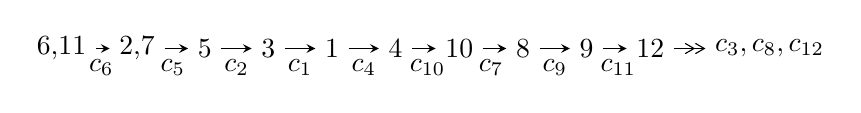
\begin{tikzpicture}[x=23pt, y=7pt]
	% node
	\node (A0) at (-1/8, 0) {6,11};
	\node (A1) at (17/16, 0) {2,7};
	\node (A2) at (17/8, 0) {5};
	\node (A3) at (25/8, 0) {3};
	\node (A4) at (33/8, 0) {1};
	\node (A5) at (41/8, 0) {4};
	\node (A6) at (49/8, 0) {10};
	\node (A7) at (57/8, 0) {8};
	\node (A8) at (65/8, 0) {9};
	\node (A9) at (73/8, 0) {12};
	\node (C1) at (1/2, -1) {$c_{6}$};
	\node (C2) at (13/8, -1) {$c_{5}$};
	\node (C3) at (21/8, -1) {$c_{2}$};
	\node (C4) at (29/8, -1) {$c_{1}$};
	\node (C5) at (37/8, -1) {$c_{4}$};
	\node (C6) at (45/8, -1) {$c_{10}$};
	\node (C7) at (53/8, -1) {$c_{7}$};
	\node (C8) at (61/8, -1) {$c_{9}$};
	\node (C9) at (69/8, -1) {$c_{11}$};
	\node (A10) at (11, 0) {$c_{3},c_{8},c_{12}$};

	% edge
	\draw[->,>=stealth]	
	(A0) edge (A1) (A1) edge (A2) (A2) edge (A3) (A3) edge (A4) (A4) edge (A5) (A5) edge (A6) (A6) edge (A7) (A7) edge (A8) (A8) edge (A9) ;
	\draw[->>,>={angle 60}]	
	(A9) edge (A10);
\end{tikzpicture} \\ 

\end{tabular} \\

\footnotetext{
The image of knot diagram is generated by the software ``\textbf{Draw programme}" developed by Andrew Bartholomew(\url{http://www.layer8.co.uk/maths/draw/index.htm\#Running-draw}), where we modified some parts for our purpose(\url{https://github.com/CATsTAILs/LinksPainter}).
}\phantom \\ \newline 
\centering \textbf{Ideals for irreducible components\footnotemark of $X_{\text{par}}$} 
 
\begin{align*}
I^u_{1}&=\langle 
159 u^{20}-349 u^{19}+\cdots+1024 b+97,\;65 u^{20}-195 u^{19}+\cdots+2048 a+2111,\;u^{21}-2 u^{20}+\cdots+5 u^2-1\rangle \\
I^u_{2}&=\langle 
2 u^7+5 u^6+11 u^5+22 u^4+25 u^3+24 u^2+7 b+15 u+1,\\
\phantom{I^u_{2}}&\phantom{= \langle  }-19 u^7-36 u^6-87 u^5-172 u^4-186 u^3-164 u^2+14 a-133 u-3,\\
\phantom{I^u_{2}}&\phantom{= \langle  }u^8+2 u^7+5 u^6+10 u^5+12 u^4+12 u^3+11 u^2+3 u+2\rangle \\
I^u_{3}&=\langle 
- a^2+2 a u+b+2 a-2 u-1,\;a^4-3 a^3 u-4 a^3+9 a^2 u+5 a^2-11 a u-2 a+5 u+1,\;u^2+1\rangle \\
I^u_{4}&=\langle 
3642 u^{11}+10715 u^{10}+\cdots+16346 b+454,\;-9302 u^{11}+5482 u^{10}+\cdots+277882 a-125487,\\
\phantom{I^u_{4}}&\phantom{= \langle  }u^{12}+3 u^{11}+11 u^{10}+23 u^9+46 u^8+68 u^7+94 u^6+99 u^5+97 u^4+76 u^3+52 u^2+26 u+17\rangle \\
I^u_{5}&=\langle 
b+2 a+2,\;4 a^2+10 a+7,\;u+1\rangle \\
\\
\end{align*}
\raggedright * 5 irreducible components of $\dim_{\mathbb{C}}=0$, with total 51 representations.\\
\footnotetext{All coefficients of polynomials are rational numbers. But the coefficients are sometimes approximated in decimal forms when there is not enough margin.}
\newpage
\renewcommand{\arraystretch}{1}
\centering \section*{I. $I^u_{1}= \langle 159 u^{20}-349 u^{19}+\cdots+1024 b+97,\;65 u^{20}-195 u^{19}+\cdots+2048 a+2111,\;u^{21}-2 u^{20}+\cdots+5 u^2-1 \rangle$}
\flushleft \textbf{(i) Arc colorings}\\
\begin{tabular}{m{7pt} m{180pt} m{7pt} m{180pt} }
\flushright $a_{6}=$&$\begin{pmatrix}1\\0\end{pmatrix}$ \\
\flushright $a_{11}=$&$\begin{pmatrix}0\\u\end{pmatrix}$ \\
\flushright $a_{2}=$&$\begin{pmatrix}-0.0317383 u^{20}+0.0952148 u^{19}+\cdots+6.03076 u-1.03076\\-0.155273 u^{20}+0.340820 u^{19}+\cdots+0.219727 u-0.0947266\end{pmatrix}$ \\
\flushright $a_{7}=$&$\begin{pmatrix}1\\- u^2\end{pmatrix}$ \\
\flushright $a_{5}=$&$\begin{pmatrix}-0.395996 u^{20}+0.992676 u^{19}+\cdots+0.588379 u+0.591309\\0.114258 u^{20}-0.327148 u^{19}+\cdots+0.583008 u-0.442383\end{pmatrix}$ \\
\flushright $a_{3}=$&$\begin{pmatrix}-0.340332 u^{20}+0.810059 u^{19}+\cdots+1.36279 u+0.301270\\0.106445 u^{20}-0.0537109 u^{19}+\cdots+0.825195 u-0.684570\end{pmatrix}$ \\
\flushright $a_{1}=$&$\begin{pmatrix}u\\0.0312500 u^{20}-0.0312500 u^{19}+\cdots+0.968750 u-0.0312500\end{pmatrix}$ \\
\flushright $a_{4}=$&$\begin{pmatrix}-0.281738 u^{20}+0.665527 u^{19}+\cdots+1.17139 u+0.148926\\0.114258 u^{20}-0.327148 u^{19}+\cdots+0.583008 u-0.442383\end{pmatrix}$ \\
\flushright $a_{10}=$&$\begin{pmatrix}- u\\u^3+u\end{pmatrix}$ \\
\flushright $a_{8}=$&$\begin{pmatrix}u^2+1\\- u^4-2 u^2\end{pmatrix}$ \\
\flushright $a_{9}=$&$\begin{pmatrix}-1\\0.0312500 u^{20}-0.0937500 u^{19}+\cdots-0.0312500 u+0.0312500\end{pmatrix}$ \\
\flushright $a_{12}=$&$\begin{pmatrix}u\\0.0312500 u^{20}-0.0312500 u^{19}+\cdots+0.968750 u-0.0312500\end{pmatrix}$\\&\end{tabular}
\flushleft \textbf{(ii) Obstruction class $= -1$}\\~\\
\flushleft \textbf{(iii) Cusp Shapes $= \frac{9279}{4096} u^{20}-\frac{13821}{4096} u^{19}+\cdots+\frac{13503}{4096} u+\frac{26625}{4096}$}\\~\\
\newpage\renewcommand{\arraystretch}{1}
\flushleft \textbf{(iv) u-Polynomials at the component}\newline \\
\begin{tabular}{m{50pt}|m{274pt}}
Crossings & \hspace{64pt}u-Polynomials at each crossing \\
\hline $$\begin{aligned}c_{1},c_{4}\end{aligned}$$&$\begin{aligned}
&u^{21}+8 u^{20}+\cdots+145 u-16
\end{aligned}$\\
\hline $$\begin{aligned}c_{2},c_{5}\end{aligned}$$&$\begin{aligned}
&u^{21}+2 u^{20}+\cdots+9 u-4
\end{aligned}$\\
\hline $$\begin{aligned}c_{3},c_{9}\end{aligned}$$&$\begin{aligned}
&u^{21}+3 u^{20}+\cdots-8 u-32
\end{aligned}$\\
\hline $$\begin{aligned}c_{6},c_{7},c_{8}\\c_{10},c_{11}\end{aligned}$$&$\begin{aligned}
&u^{21}-2 u^{20}+\cdots+5 u^2-1
\end{aligned}$\\
\hline $$\begin{aligned}c_{12}\end{aligned}$$&$\begin{aligned}
&u^{21}+26 u^{20}+\cdots+10 u-1
\end{aligned}$\\
\hline
\end{tabular}\\~\\
\newpage\renewcommand{\arraystretch}{1}
\flushleft \textbf{(v) Riley Polynomials at the component}\newline \\
\begin{tabular}{m{50pt}|m{274pt}}
Crossings & \hspace{64pt}Riley Polynomials at each crossing \\
\hline $$\begin{aligned}c_{1},c_{4}\end{aligned}$$&$\begin{aligned}
&y^{21}+12 y^{20}+\cdots+51681 y-256
\end{aligned}$\\
\hline $$\begin{aligned}c_{2},c_{5}\end{aligned}$$&$\begin{aligned}
&y^{21}+8 y^{20}+\cdots+145 y-16
\end{aligned}$\\
\hline $$\begin{aligned}c_{3},c_{9}\end{aligned}$$&$\begin{aligned}
&y^{21}-5 y^{20}+\cdots-4928 y-1024
\end{aligned}$\\
\hline $$\begin{aligned}c_{6},c_{7},c_{8}\\c_{10},c_{11}\end{aligned}$$&$\begin{aligned}
&y^{21}+26 y^{20}+\cdots+10 y-1
\end{aligned}$\\
\hline $$\begin{aligned}c_{12}\end{aligned}$$&$\begin{aligned}
&y^{21}-66 y^{20}+\cdots+126 y-1
\end{aligned}$\\
\hline
\end{tabular}\\~\\
\newpage\flushleft \textbf{(vi) Complex Volumes and Cusp Shapes}
$$\begin{array}{c|c|c}  
\text{Solutions to }I^u_{1}& \I (\text{vol} + \sqrt{-1}CS) & \text{Cusp shape}\\
 \hline 
\begin{aligned}
u &= \phantom{-}0.458142 + 0.833548 I \\
a &= \phantom{-}0.677568 - 0.339414 I \\
b &= -0.773041 + 0.928850 I\end{aligned}
 & \phantom{-}4.17175 - 1.61049 I & \phantom{-}8.87690 - 1.72492 I \\ \hline\begin{aligned}
u &= \phantom{-}0.458142 - 0.833548 I \\
a &= \phantom{-}0.677568 + 0.339414 I \\
b &= -0.773041 - 0.928850 I\end{aligned}
 & \phantom{-}4.17175 + 1.61049 I & \phantom{-}8.87690 + 1.72492 I \\ \hline\begin{aligned}
u &= \phantom{-}0.334381 + 0.773560 I \\
a &= \phantom{-}1.290350 - 0.376146 I \\
b &= -0.805389 - 0.873526 I\end{aligned}
 & \phantom{-}4.35172 + 4.34513 I & \phantom{-}10.07573 - 8.03255 I \\ \hline\begin{aligned}
u &= \phantom{-}0.334381 - 0.773560 I \\
a &= \phantom{-}1.290350 + 0.376146 I \\
b &= -0.805389 + 0.873526 I\end{aligned}
 & \phantom{-}4.35172 - 4.34513 I & \phantom{-}10.07573 + 8.03255 I \\ \hline\begin{aligned}
u &= \phantom{-}1.216790 + 0.212353 I \\
a &= \phantom{-}1.211710 + 0.267891 I \\
b &= -0.377864 - 0.854536 I\end{aligned}
 & \phantom{-}1.30694 + 1.63824 I & -1.29573 + 4.22399 I \\ \hline\begin{aligned}
u &= \phantom{-}1.216790 - 0.212353 I \\
a &= \phantom{-}1.211710 - 0.267891 I \\
b &= -0.377864 + 0.854536 I\end{aligned}
 & \phantom{-}1.30694 - 1.63824 I & -1.29573 - 4.22399 I \\ \hline\begin{aligned}
u &= \phantom{-}0.097170 + 0.403788 I \\
a &= \phantom{-}0.57317 + 1.41705 I \\
b &= \phantom{-}0.207107 + 0.829659 I\end{aligned}
 & -1.22812 + 1.66803 I & \phantom{-}2.33962 - 5.96953 I \\ \hline\begin{aligned}
u &= \phantom{-}0.097170 - 0.403788 I \\
a &= \phantom{-}0.57317 - 1.41705 I \\
b &= \phantom{-}0.207107 - 0.829659 I\end{aligned}
 & -1.22812 - 1.66803 I & \phantom{-}2.33962 + 5.96953 I \\ \hline\begin{aligned}
u &= \phantom{-}0.381501\phantom{ +0.000000I} \\
a &= \phantom{-}0.337636\phantom{ +0.000000I} \\
b &= \phantom{-}0.264712\phantom{ +0.000000I}\end{aligned}
 & \phantom{-}0.708376\phantom{ +0.000000I} & \phantom{-}14.4470\phantom{ +0.000000I} \\ \hline\begin{aligned}
u &= -0.02913 + 1.62816 I \\
a &= -0.961297 + 0.342959 I \\
b &= \phantom{-}1.038150 - 0.513588 I\end{aligned}
 & -10.09800 - 1.80625 I & \phantom{-}3.06957 + 1.66115 I\\
 \hline 
 \end{array}$$\newpage$$\begin{array}{c|c|c}  
\text{Solutions to }I^u_{1}& \I (\text{vol} + \sqrt{-1}CS) & \text{Cusp shape}\\
 \hline 
\begin{aligned}
u &= -0.02913 - 1.62816 I \\
a &= -0.961297 - 0.342959 I \\
b &= \phantom{-}1.038150 + 0.513588 I\end{aligned}
 & -10.09800 + 1.80625 I & \phantom{-}3.06957 - 1.66115 I \\ \hline\begin{aligned}
u &= -0.38269 + 1.61174 I \\
a &= \phantom{-}0.856171 + 0.551613 I \\
b &= -1.005420 - 0.467651 I\end{aligned}
 & -10.43370 - 7.89166 I & \phantom{-}3.87913 + 3.10640 I \\ \hline\begin{aligned}
u &= -0.38269 - 1.61174 I \\
a &= \phantom{-}0.856171 - 0.551613 I \\
b &= -1.005420 + 0.467651 I\end{aligned}
 & -10.43370 + 7.89166 I & \phantom{-}3.87913 - 3.10640 I \\ \hline\begin{aligned}
u &= \phantom{-}0.10115 + 1.67309 I \\
a &= -1.266450 + 0.124462 I \\
b &= \phantom{-}0.725547 + 1.193790 I\end{aligned}
 & -12.24280 + 4.61265 I & \phantom{-}1.46303 - 2.55091 I \\ \hline\begin{aligned}
u &= \phantom{-}0.10115 - 1.67309 I \\
a &= -1.266450 - 0.124462 I \\
b &= \phantom{-}0.725547 - 1.193790 I\end{aligned}
 & -12.24280 - 4.61265 I & \phantom{-}1.46303 + 2.55091 I \\ \hline\begin{aligned}
u &= -0.49023 + 1.63779 I \\
a &= \phantom{-}1.53317 + 0.26133 I \\
b &= -0.694270 + 1.177460 I\end{aligned}
 & -12.6524 - 14.0619 I & \phantom{-}2.23345 + 6.95334 I \\ \hline\begin{aligned}
u &= -0.49023 - 1.63779 I \\
a &= \phantom{-}1.53317 - 0.26133 I \\
b &= -0.694270 - 1.177460 I\end{aligned}
 & -12.6524 + 14.0619 I & \phantom{-}2.23345 - 6.95334 I \\ \hline\begin{aligned}
u &= -0.265665 + 0.100260 I \\
a &= -3.22189 + 1.30088 I \\
b &= \phantom{-}0.565254 - 0.857227 I\end{aligned}
 & \phantom{-}0.38970 - 2.24826 I & \phantom{-}1.51589 + 3.88242 I \\ \hline\begin{aligned}
u &= -0.265665 - 0.100260 I \\
a &= -3.22189 - 1.30088 I \\
b &= \phantom{-}0.565254 + 0.857227 I\end{aligned}
 & \phantom{-}0.38970 + 2.24826 I & \phantom{-}1.51589 - 3.88242 I \\ \hline\begin{aligned}
u &= -0.23068 + 1.77893 I \\
a &= -0.111321 - 0.270180 I \\
b &= -0.012425 - 1.345530 I\end{aligned}
 & -17.3796 - 4.8017 I & -0.50589 + 2.16688 I\\
 \hline 
 \end{array}$$\newpage$$\begin{array}{c|c|c}  
\text{Solutions to }I^u_{1}& \I (\text{vol} + \sqrt{-1}CS) & \text{Cusp shape}\\
 \hline 
\begin{aligned}
u &= -0.23068 - 1.77893 I \\
a &= -0.111321 + 0.270180 I \\
b &= -0.012425 + 1.345530 I\end{aligned}
 & -17.3796 + 4.8017 I & -0.50589 - 2.16688 I\\
 \hline 
 \end{array}$$\newpage\newpage\renewcommand{\arraystretch}{1}
\centering \section*{II. $I^u_{2}= \langle 2 u^7+5 u^6+\cdots+7 b+1,\;-19 u^7-36 u^6+\cdots+14 a-3,\;u^8+2 u^7+\cdots+3 u+2 \rangle$}
\flushleft \textbf{(i) Arc colorings}\\
\begin{tabular}{m{7pt} m{180pt} m{7pt} m{180pt} }
\flushright $a_{6}=$&$\begin{pmatrix}1\\0\end{pmatrix}$ \\
\flushright $a_{11}=$&$\begin{pmatrix}0\\u\end{pmatrix}$ \\
\flushright $a_{2}=$&$\begin{pmatrix}\frac{19}{14} u^7+\frac{18}{7} u^6+\cdots+\frac{19}{2} u+\frac{3}{14}\\-\frac{2}{7} u^7-\frac{5}{7} u^6+\cdots-\frac{15}{7} u-\frac{1}{7}\end{pmatrix}$ \\
\flushright $a_{7}=$&$\begin{pmatrix}1\\- u^2\end{pmatrix}$ \\
\flushright $a_{5}=$&$\begin{pmatrix}0.785714 u^{7}+1.71429 u^{6}+\cdots+8.64286 u+3.64286\\-\frac{2}{7} u^7-\frac{4}{7} u^6+\cdots-\frac{16}{7} u-\frac{5}{7}\end{pmatrix}$ \\
\flushright $a_{3}=$&$\begin{pmatrix}u^7+\frac{16}{7} u^6+\cdots+\frac{75}{7} u+\frac{20}{7}\\-\frac{2}{7} u^7-\frac{6}{7} u^6+\cdots-3 u-\frac{4}{7}\end{pmatrix}$ \\
\flushright $a_{1}=$&$\begin{pmatrix}0.785714 u^{7}+1.57143 u^{6}+\cdots+7.78571 u+2.21429\\-\frac{2}{7} u^7-\frac{4}{7} u^6+\cdots-\frac{16}{7} u-\frac{5}{7}\end{pmatrix}$ \\
\flushright $a_{4}=$&$\begin{pmatrix}\frac{1}{2} u^7+\frac{8}{7} u^6+\cdots+\frac{89}{14} u+\frac{41}{14}\\-\frac{2}{7} u^7-\frac{4}{7} u^6+\cdots-\frac{16}{7} u-\frac{5}{7}\end{pmatrix}$ \\
\flushright $a_{10}=$&$\begin{pmatrix}- u\\u^3+u\end{pmatrix}$ \\
\flushright $a_{8}=$&$\begin{pmatrix}u^2+1\\- u^4-2 u^2\end{pmatrix}$ \\
\flushright $a_{9}=$&$\begin{pmatrix}-\frac{5}{14} u^7-\frac{3}{7} u^6+\cdots-\frac{9}{14} u+\frac{31}{14}\\-\frac{1}{7} u^6-\frac{2}{7} u^4+\cdots+\frac{1}{7} u-\frac{3}{7}\end{pmatrix}$ \\
\flushright $a_{12}=$&$\begin{pmatrix}0.785714 u^{7}+1.57143 u^{6}+\cdots+7.78571 u+2.21429\\-\frac{3}{7} u^7-\frac{4}{7} u^6+\cdots-\frac{5}{7} u-\frac{5}{7}\end{pmatrix}$\\&\end{tabular}
\flushleft \textbf{(ii) Obstruction class $= -1$}\\~\\
\flushleft \textbf{(iii) Cusp Shapes $= \frac{8}{7} u^7+\frac{20}{7} u^6+\frac{44}{7} u^5+\frac{88}{7} u^4+\frac{128}{7} u^3+\frac{96}{7} u^2+\frac{88}{7} u+\frac{74}{7}$}\\~\\
\newpage\renewcommand{\arraystretch}{1}
\flushleft \textbf{(iv) u-Polynomials at the component}\newline \\
\begin{tabular}{m{50pt}|m{274pt}}
Crossings & \hspace{64pt}u-Polynomials at each crossing \\
\hline $$\begin{aligned}c_{1},c_{4}\end{aligned}$$&$\begin{aligned}
&(u^4+2 u^3+3 u^2+u+1)^2
\end{aligned}$\\
\hline $$\begin{aligned}c_{2},c_{5}\end{aligned}$$&$\begin{aligned}
&(u^4+u^2- u+1)^2
\end{aligned}$\\
\hline $$\begin{aligned}c_{3},c_{9}\end{aligned}$$&$\begin{aligned}
&(u^4+u^2+u+1)^2
\end{aligned}$\\
\hline $$\begin{aligned}c_{6},c_{7},c_{8}\\c_{10},c_{11}\end{aligned}$$&$\begin{aligned}
&u^8+2 u^7+5 u^6+10 u^5+12 u^4+12 u^3+11 u^2+3 u+2
\end{aligned}$\\
\hline $$\begin{aligned}c_{12}\end{aligned}$$&$\begin{aligned}
&u^8+6 u^7+9 u^6-6 u^5+6 u^4+80 u^3+97 u^2+35 u+4
\end{aligned}$\\
\hline
\end{tabular}\\~\\
\newpage\renewcommand{\arraystretch}{1}
\flushleft \textbf{(v) Riley Polynomials at the component}\newline \\
\begin{tabular}{m{50pt}|m{274pt}}
Crossings & \hspace{64pt}Riley Polynomials at each crossing \\
\hline $$\begin{aligned}c_{1},c_{4}\end{aligned}$$&$\begin{aligned}
&(y^4+2 y^3+7 y^2+5 y+1)^2
\end{aligned}$\\
\hline $$\begin{aligned}c_{2},c_{3},c_{5}\\c_{9}\end{aligned}$$&$\begin{aligned}
&(y^4+2 y^3+3 y^2+y+1)^2
\end{aligned}$\\
\hline $$\begin{aligned}c_{6},c_{7},c_{8}\\c_{10},c_{11}\end{aligned}$$&$\begin{aligned}
&y^8+6 y^7+9 y^6-6 y^5+6 y^4+80 y^3+97 y^2+35 y+4
\end{aligned}$\\
\hline $$\begin{aligned}c_{12}\end{aligned}$$&$\begin{aligned}
&y^8-18 y^7+\cdots-449 y+16
\end{aligned}$\\
\hline
\end{tabular}\\~\\
\newpage\flushleft \textbf{(vi) Complex Volumes and Cusp Shapes}
$$\begin{array}{c|c|c}  
\text{Solutions to }I^u_{2}& \I (\text{vol} + \sqrt{-1}CS) & \text{Cusp shape}\\
 \hline 
\begin{aligned}
u &= \phantom{-}0.003353 + 1.153470 I \\
a &= \phantom{-}0.283780 - 0.486090 I \\
b &= \phantom{-}0.547424 + 0.585652 I\end{aligned}
 & -2.30977 + 1.39709 I & \phantom{-}7.77019 - 3.86736 I \\ \hline\begin{aligned}
u &= \phantom{-}0.003353 - 1.153470 I \\
a &= \phantom{-}0.283780 + 0.486090 I \\
b &= \phantom{-}0.547424 - 0.585652 I\end{aligned}
 & -2.30977 - 1.39709 I & \phantom{-}7.77019 + 3.86736 I \\ \hline\begin{aligned}
u &= -1.281480 + 0.482756 I \\
a &= \phantom{-}1.44914 - 0.47651 I \\
b &= -0.547424 + 1.120870 I\end{aligned}
 & -5.91490 - 7.64338 I & \phantom{-}2.22981 + 6.51087 I \\ \hline\begin{aligned}
u &= -1.281480 - 0.482756 I \\
a &= \phantom{-}1.44914 + 0.47651 I \\
b &= -0.547424 - 1.120870 I\end{aligned}
 & -5.91490 + 7.64338 I & \phantom{-}2.22981 - 6.51087 I \\ \hline\begin{aligned}
u &= -0.046668 + 0.512275 I \\
a &= -2.11815 + 3.03669 I \\
b &= \phantom{-}0.547424 - 0.585652 I\end{aligned}
 & -2.30977 - 1.39709 I & \phantom{-}7.77019 + 3.86736 I \\ \hline\begin{aligned}
u &= -0.046668 - 0.512275 I \\
a &= -2.11815 - 3.03669 I \\
b &= \phantom{-}0.547424 + 0.585652 I\end{aligned}
 & -2.30977 + 1.39709 I & \phantom{-}7.77019 - 3.86736 I \\ \hline\begin{aligned}
u &= \phantom{-}0.32480 + 1.70994 I \\
a &= \phantom{-}1.135230 - 0.382122 I \\
b &= -0.547424 - 1.120870 I\end{aligned}
 & -5.91490 + 7.64338 I & \phantom{-}2.22981 - 6.51087 I \\ \hline\begin{aligned}
u &= \phantom{-}0.32480 - 1.70994 I \\
a &= \phantom{-}1.135230 + 0.382122 I \\
b &= -0.547424 + 1.120870 I\end{aligned}
 & -5.91490 - 7.64338 I & \phantom{-}2.22981 + 6.51087 I\\
 \hline 
 \end{array}$$\newpage\newpage\renewcommand{\arraystretch}{1}
\centering \section*{III. $I^u_{3}= \langle - a^2+2 a u+b+2 a-2 u-1,\;-3 a^3 u+9 a^2 u+\cdots-2 a+1,\;u^2+1 \rangle$}
\flushleft \textbf{(i) Arc colorings}\\
\begin{tabular}{m{7pt} m{180pt} m{7pt} m{180pt} }
\flushright $a_{6}=$&$\begin{pmatrix}1\\0\end{pmatrix}$ \\
\flushright $a_{11}=$&$\begin{pmatrix}0\\u\end{pmatrix}$ \\
\flushright $a_{2}=$&$\begin{pmatrix}a\\a^2-2 a u-2 a+2 u+1\end{pmatrix}$ \\
\flushright $a_{7}=$&$\begin{pmatrix}1\\1\end{pmatrix}$ \\
\flushright $a_{5}=$&$\begin{pmatrix}a^3-2 a^2 u-2 a^2+2 a u+a+1\\- a^3 u+3 a^2 u-3 a^2- a u+6 a- u-4\end{pmatrix}$ \\
\flushright $a_{3}=$&$\begin{pmatrix}- a^3 u+4 a^2 u-2 a^2-5 a u+6 a+3 u-4\\a^3 u-3 a^2 u+4 a^2-8 a+2 u+6\end{pmatrix}$ \\
\flushright $a_{1}=$&$\begin{pmatrix}u\\a u- u+2\end{pmatrix}$ \\
\flushright $a_{4}=$&$\begin{pmatrix}- a^3 u+a^3+a^2 u-5 a^2+a u+7 a- u-3\\- a^3 u+3 a^2 u-3 a^2- a u+6 a- u-4\end{pmatrix}$ \\
\flushright $a_{10}=$&$\begin{pmatrix}- u\\0\end{pmatrix}$ \\
\flushright $a_{8}=$&$\begin{pmatrix}0\\1\end{pmatrix}$ \\
\flushright $a_{9}=$&$\begin{pmatrix}-1\\- a+2 u+1\end{pmatrix}$ \\
\flushright $a_{12}=$&$\begin{pmatrix}u\\a u+2\end{pmatrix}$\\&\end{tabular}
\flushleft \textbf{(ii) Obstruction class $= 1$}\\~\\
\flushleft \textbf{(iii) Cusp Shapes $= 4 a^3 u-12 a^2 u+8 a^2+12 a u-16 a-4 u+12$}\\~\\
\newpage\renewcommand{\arraystretch}{1}
\flushleft \textbf{(iv) u-Polynomials at the component}\newline \\
\begin{tabular}{m{50pt}|m{274pt}}
Crossings & \hspace{64pt}u-Polynomials at each crossing \\
\hline $$\begin{aligned}c_{1},c_{4}\end{aligned}$$&$\begin{aligned}
&(u^4- u^3+3 u^2-2 u+1)^2
\end{aligned}$\\
\hline $$\begin{aligned}c_{2}\end{aligned}$$&$\begin{aligned}
&(u^4- u^3+u^2+1)^2
\end{aligned}$\\
\hline $$\begin{aligned}c_{3},c_{9}\end{aligned}$$&$\begin{aligned}
&u^8-5 u^6+7 u^4-2 u^2+1
\end{aligned}$\\
\hline $$\begin{aligned}c_{5}\end{aligned}$$&$\begin{aligned}
&(u^4+u^3+u^2+1)^2
\end{aligned}$\\
\hline $$\begin{aligned}c_{6},c_{7},c_{8}\\c_{10},c_{11}\end{aligned}$$&$\begin{aligned}
&(u^2+1)^4
\end{aligned}$\\
\hline $$\begin{aligned}c_{12}\end{aligned}$$&$\begin{aligned}
&(u+1)^8
\end{aligned}$\\
\hline
\end{tabular}\\~\\
\newpage\renewcommand{\arraystretch}{1}
\flushleft \textbf{(v) Riley Polynomials at the component}\newline \\
\begin{tabular}{m{50pt}|m{274pt}}
Crossings & \hspace{64pt}Riley Polynomials at each crossing \\
\hline $$\begin{aligned}c_{1},c_{4}\end{aligned}$$&$\begin{aligned}
&(y^4+5 y^3+7 y^2+2 y+1)^2
\end{aligned}$\\
\hline $$\begin{aligned}c_{2},c_{5}\end{aligned}$$&$\begin{aligned}
&(y^4+y^3+3 y^2+2 y+1)^2
\end{aligned}$\\
\hline $$\begin{aligned}c_{3},c_{9}\end{aligned}$$&$\begin{aligned}
&(y^4-5 y^3+7 y^2-2 y+1)^2
\end{aligned}$\\
\hline $$\begin{aligned}c_{6},c_{7},c_{8}\\c_{10},c_{11}\end{aligned}$$&$\begin{aligned}
&(y+1)^8
\end{aligned}$\\
\hline $$\begin{aligned}c_{12}\end{aligned}$$&$\begin{aligned}
&(y-1)^8
\end{aligned}$\\
\hline
\end{tabular}\\~\\
\newpage\flushleft \textbf{(vi) Complex Volumes and Cusp Shapes}
$$\begin{array}{c|c|c}  
\text{Solutions to }I^u_{3}& \I (\text{vol} + \sqrt{-1}CS) & \text{Cusp shape}\\
 \hline 
\begin{aligned}
u &= \phantom{-0.000000 -}1.000000 I \\
a &= \phantom{-}0.674360 - 0.399232 I \\
b &= -0.851808 + 0.911292 I\end{aligned}
 & \phantom{-}3.50087 - 3.16396 I & \phantom{-}3.82674 + 2.56480 I \\ \hline\begin{aligned}
u &= \phantom{-0.000000 -}1.000000 I \\
a &= \phantom{-}1.325640 - 0.399232 I \\
b &= -0.851808 - 0.911292 I\end{aligned}
 & \phantom{-}3.50087 + 3.16396 I & \phantom{-}3.82674 - 2.56480 I \\ \hline\begin{aligned}
u &= \phantom{-0.000000 -}1.000000 I \\
a &= \phantom{-}0.59947 + 1.89923 I \\
b &= \phantom{-}0.351808 - 0.720342 I\end{aligned}
 & -3.50087 - 1.41510 I & \phantom{-}0.17326 + 4.90874 I \\ \hline\begin{aligned}
u &= \phantom{-0.000000 -}1.000000 I \\
a &= \phantom{-}1.40053 + 1.89923 I \\
b &= \phantom{-}0.351808 + 0.720342 I\end{aligned}
 & -3.50087 + 1.41510 I & \phantom{-}0.17326 - 4.90874 I \\ \hline\begin{aligned}
u &= \phantom{-0.000000 } -1.000000 I \\
a &= \phantom{-}0.674360 + 0.399232 I \\
b &= -0.851808 - 0.911292 I\end{aligned}
 & \phantom{-}3.50087 + 3.16396 I & \phantom{-}3.82674 - 2.56480 I \\ \hline\begin{aligned}
u &= \phantom{-0.000000 } -1.000000 I \\
a &= \phantom{-}1.325640 + 0.399232 I \\
b &= -0.851808 + 0.911292 I\end{aligned}
 & \phantom{-}3.50087 - 3.16396 I & \phantom{-}3.82674 + 2.56480 I \\ \hline\begin{aligned}
u &= \phantom{-0.000000 } -1.000000 I \\
a &= \phantom{-}0.59947 - 1.89923 I \\
b &= \phantom{-}0.351808 + 0.720342 I\end{aligned}
 & -3.50087 + 1.41510 I & \phantom{-}0.17326 - 4.90874 I \\ \hline\begin{aligned}
u &= \phantom{-0.000000 } -1.000000 I \\
a &= \phantom{-}1.40053 - 1.89923 I \\
b &= \phantom{-}0.351808 - 0.720342 I\end{aligned}
 & -3.50087 - 1.41510 I & \phantom{-}0.17326 + 4.90874 I\\
 \hline 
 \end{array}$$\newpage\newpage\renewcommand{\arraystretch}{1}
\centering \section*{IV. $I^u_{4}= \langle 3642 u^{11}+10715 u^{10}+\cdots+16346 b+454,\;-9302 u^{11}+5482 u^{10}+\cdots+277882 a-125487,\;u^{12}+3 u^{11}+\cdots+26 u+17 \rangle$}
\flushleft \textbf{(i) Arc colorings}\\
\begin{tabular}{m{7pt} m{180pt} m{7pt} m{180pt} }
\flushright $a_{6}=$&$\begin{pmatrix}1\\0\end{pmatrix}$ \\
\flushright $a_{11}=$&$\begin{pmatrix}0\\u\end{pmatrix}$ \\
\flushright $a_{2}=$&$\begin{pmatrix}0.0334746 u^{11}-0.0197278 u^{10}+\cdots+2.00276 u+0.451584\\-0.222807 u^{11}-0.655512 u^{10}+\cdots-1.99700 u-0.0277744\end{pmatrix}$ \\
\flushright $a_{7}=$&$\begin{pmatrix}1\\- u^2\end{pmatrix}$ \\
\flushright $a_{5}=$&$\begin{pmatrix}0.128213 u^{11}+0.278557 u^{10}+\cdots-4.21560 u-3.08761\\-0.0231249 u^{11}-0.186651 u^{10}+\cdots-0.439557 u-0.366145\end{pmatrix}$ \\
\flushright $a_{3}=$&$\begin{pmatrix}0.0932842 u^{11}+0.0428527 u^{10}+\cdots-4.81556 u-3.27790\\-0.0855255 u^{11}-0.333170 u^{10}+\cdots-1.36376 u-0.854154\end{pmatrix}$ \\
\flushright $a_{1}=$&$\begin{pmatrix}0.125996 u^{11}+0.290076 u^{10}+\cdots+3.62135 u+1.59297\\-0.0671724 u^{11}-0.113606 u^{10}+\cdots-0.562523 u-0.0635630\end{pmatrix}$ \\
\flushright $a_{4}=$&$\begin{pmatrix}0.105088 u^{11}+0.0919059 u^{10}+\cdots-4.65516 u-3.45376\\-0.0231249 u^{11}-0.186651 u^{10}+\cdots-0.439557 u-0.366145\end{pmatrix}$ \\
\flushright $a_{10}=$&$\begin{pmatrix}- u\\u^3+u\end{pmatrix}$ \\
\flushright $a_{8}=$&$\begin{pmatrix}u^2+1\\- u^4-2 u^2\end{pmatrix}$ \\
\flushright $a_{9}=$&$\begin{pmatrix}-0.00373900 u^{11}+0.0559554 u^{10}+\cdots+0.431964 u+1.46531\\0.0879114 u^{11}+0.316714 u^{10}+\cdots+1.68292 u+0.141931\end{pmatrix}$ \\
\flushright $a_{12}=$&$\begin{pmatrix}0.125996 u^{11}+0.290076 u^{10}+\cdots+3.62135 u+1.59297\\-0.0141931 u^{11}-0.0431298 u^{10}+\cdots-0.706289 u-1.55806\end{pmatrix}$\\&\end{tabular}
\flushleft \textbf{(ii) Obstruction class $= -1$}\\~\\
\flushleft \textbf{(iii) Cusp Shapes $= \frac{2796}{8173} u^{11}+\frac{10892}{8173} u^{10}+\frac{36956}{8173} u^9+\frac{76592}{8173} u^8+\frac{143424}{8173} u^7+\frac{188928}{8173} u^6+\frac{226188}{8173} u^5+\frac{193280}{8173} u^4+\frac{144560}{8173} u^3+\frac{67608}{8173} u^2+\frac{44584}{8173} u+\frac{44270}{8173}$}\\~\\
\newpage\renewcommand{\arraystretch}{1}
\flushleft \textbf{(iv) u-Polynomials at the component}\newline \\
\begin{tabular}{m{50pt}|m{274pt}}
Crossings & \hspace{64pt}u-Polynomials at each crossing \\
\hline $$\begin{aligned}c_{1},c_{4}\end{aligned}$$&$\begin{aligned}
&(u^6+3 u^5+4 u^4+2 u^3+1)^2
\end{aligned}$\\
\hline $$\begin{aligned}c_{2},c_{5}\end{aligned}$$&$\begin{aligned}
&(u^6+u^5+2 u^4+2 u^3+2 u^2+2 u+1)^2
\end{aligned}$\\
\hline $$\begin{aligned}c_{3},c_{9}\end{aligned}$$&$\begin{aligned}
&(u^6- u^5+2 u^4-2 u^3+2 u^2-2 u+1)^2
\end{aligned}$\\
\hline $$\begin{aligned}c_{6},c_{7},c_{8}\\c_{10},c_{11}\end{aligned}$$&$\begin{aligned}
&u^{12}+3 u^{11}+\cdots+26 u+17
\end{aligned}$\\
\hline $$\begin{aligned}c_{12}\end{aligned}$$&$\begin{aligned}
&u^{12}+13 u^{11}+\cdots+1092 u+289
\end{aligned}$\\
\hline
\end{tabular}\\~\\
\newpage\renewcommand{\arraystretch}{1}
\flushleft \textbf{(v) Riley Polynomials at the component}\newline \\
\begin{tabular}{m{50pt}|m{274pt}}
Crossings & \hspace{64pt}Riley Polynomials at each crossing \\
\hline $$\begin{aligned}c_{1},c_{4}\end{aligned}$$&$\begin{aligned}
&(y^6- y^5+4 y^4-2 y^3+8 y^2+1)^2
\end{aligned}$\\
\hline $$\begin{aligned}c_{2},c_{3},c_{5}\\c_{9}\end{aligned}$$&$\begin{aligned}
&(y^6+3 y^5+4 y^4+2 y^3+1)^2
\end{aligned}$\\
\hline $$\begin{aligned}c_{6},c_{7},c_{8}\\c_{10},c_{11}\end{aligned}$$&$\begin{aligned}
&y^{12}+13 y^{11}+\cdots+1092 y+289
\end{aligned}$\\
\hline $$\begin{aligned}c_{12}\end{aligned}$$&$\begin{aligned}
&y^{12}-19 y^{11}+\cdots-7564 y+83521
\end{aligned}$\\
\hline
\end{tabular}\\~\\
\newpage\flushleft \textbf{(vi) Complex Volumes and Cusp Shapes}
$$\begin{array}{c|c|c}  
\text{Solutions to }I^u_{4}& \I (\text{vol} + \sqrt{-1}CS) & \text{Cusp shape}\\
 \hline 
\begin{aligned}
u &= -0.942355 + 0.499238 I \\
a &= \phantom{-}1.51895 + 0.47306 I \\
b &= -0.713912 - 0.305839 I\end{aligned}
 & -3.55561 - 2.82812 I & \phantom{-}5.50976 + 2.97945 I \\ \hline\begin{aligned}
u &= -0.942355 - 0.499238 I \\
a &= \phantom{-}1.51895 - 0.47306 I \\
b &= -0.713912 + 0.305839 I\end{aligned}
 & -3.55561 + 2.82812 I & \phantom{-}5.50976 - 2.97945 I \\ \hline\begin{aligned}
u &= \phantom{-}0.343993 + 0.784320 I \\
a &= -3.38338 - 0.25597 I \\
b &= \phantom{-}0.498832 + 1.001300 I\end{aligned}
 & -3.55561 + 2.82812 I & \phantom{-}5.50976 - 2.97945 I \\ \hline\begin{aligned}
u &= \phantom{-}0.343993 - 0.784320 I \\
a &= -3.38338 + 0.25597 I \\
b &= \phantom{-}0.498832 - 1.001300 I\end{aligned}
 & -3.55561 - 2.82812 I & \phantom{-}5.50976 + 2.97945 I \\ \hline\begin{aligned}
u &= \phantom{-}0.072139 + 1.221000 I \\
a &= -0.36108 - 1.66788 I \\
b &= \phantom{-}0.498832 - 1.001300 I\end{aligned}
 & -3.55561 - 2.82812 I & \phantom{-}5.50976 + 2.97945 I \\ \hline\begin{aligned}
u &= \phantom{-}0.072139 - 1.221000 I \\
a &= -0.36108 + 1.66788 I \\
b &= \phantom{-}0.498832 + 1.001300 I\end{aligned}
 & -3.55561 + 2.82812 I & \phantom{-}5.50976 - 2.97945 I \\ \hline\begin{aligned}
u &= -0.98583 + 1.05129 I \\
a &= \phantom{-}0.337035 + 0.395158 I \\
b &= -0.284920 - 1.115140 I\end{aligned}
 & -7.69319\phantom{ +0.000000I} &                  -6
-1.019511 + 0. 10   I\phantom{ +0.000000I} \\ \hline\begin{aligned}
u &= -0.98583 - 1.05129 I \\
a &= \phantom{-}0.337035 - 0.395158 I \\
b &= -0.284920 + 1.115140 I\end{aligned}
 & -7.69319\phantom{ +0.000000I} &                  -6
-1.019511 + 0. 10   I\phantom{ +0.000000I} \\ \hline\begin{aligned}
u &= \phantom{-}0.18858 + 1.49820 I \\
a &= \phantom{-}0.690257 - 0.163478 I \\
b &= -0.713912 + 0.305839 I\end{aligned}
 & -3.55561 + 2.82812 I & \phantom{-}5.50976 - 2.97945 I \\ \hline\begin{aligned}
u &= \phantom{-}0.18858 - 1.49820 I \\
a &= \phantom{-}0.690257 + 0.163478 I \\
b &= -0.713912 - 0.305839 I\end{aligned}
 & -3.55561 - 2.82812 I & \phantom{-}5.50976 + 2.97945 I\\
 \hline 
 \end{array}$$\newpage$$\begin{array}{c|c|c}  
\text{Solutions to }I^u_{4}& \I (\text{vol} + \sqrt{-1}CS) & \text{Cusp shape}\\
 \hline 
\begin{aligned}
u &= -0.17653 + 1.68674 I \\
a &= \phantom{-}0.786457 + 0.514816 I \\
b &= -0.284920 + 1.115140 I\end{aligned}
 & -7.69319\phantom{ +0.000000I} &                  -6
-1.019511 + 0. 10   I\phantom{ +0.000000I} \\ \hline\begin{aligned}
u &= -0.17653 - 1.68674 I \\
a &= \phantom{-}0.786457 - 0.514816 I \\
b &= -0.284920 - 1.115140 I\end{aligned}
 & -7.69319\phantom{ +0.000000I} &                  -6
-1.019511 + 0. 10   I\phantom{ +0.000000I}\\
 \hline 
 \end{array}$$\newpage\newpage\renewcommand{\arraystretch}{1}
\centering \section*{V. $I^u_{5}= \langle b+2 a+2,\;4 a^2+10 a+7,\;u+1 \rangle$}
\flushleft \textbf{(i) Arc colorings}\\
\begin{tabular}{m{7pt} m{180pt} m{7pt} m{180pt} }
\flushright $a_{6}=$&$\begin{pmatrix}1\\0\end{pmatrix}$ \\
\flushright $a_{11}=$&$\begin{pmatrix}0\\-1\end{pmatrix}$ \\
\flushright $a_{2}=$&$\begin{pmatrix}a\\-2 a-2\end{pmatrix}$ \\
\flushright $a_{7}=$&$\begin{pmatrix}1\\-1\end{pmatrix}$ \\
\flushright $a_{5}=$&$\begin{pmatrix}3 a+\frac{9}{2}\\-2 a-3\end{pmatrix}$ \\
\flushright $a_{3}=$&$\begin{pmatrix}a+\frac{3}{2}\\-2 a-3\end{pmatrix}$ \\
\flushright $a_{1}=$&$\begin{pmatrix}-1\\0\end{pmatrix}$ \\
\flushright $a_{4}=$&$\begin{pmatrix}a+\frac{3}{2}\\-2 a-3\end{pmatrix}$ \\
\flushright $a_{10}=$&$\begin{pmatrix}1\\-2\end{pmatrix}$ \\
\flushright $a_{8}=$&$\begin{pmatrix}2\\-3\end{pmatrix}$ \\
\flushright $a_{9}=$&$\begin{pmatrix}1\\-2\end{pmatrix}$ \\
\flushright $a_{12}=$&$\begin{pmatrix}-1\\1\end{pmatrix}$\\&\end{tabular}
\flushleft \textbf{(ii) Obstruction class $= 1$}\\~\\
\flushleft \textbf{(iii) Cusp Shapes $= \frac{31}{2} a+\frac{59}{2}$}\\~\\
\newpage\renewcommand{\arraystretch}{1}
\flushleft \textbf{(iv) u-Polynomials at the component}\newline \\
\begin{tabular}{m{50pt}|m{274pt}}
Crossings & \hspace{64pt}u-Polynomials at each crossing \\
\hline $$\begin{aligned}c_{1},c_{4},c_{5}\end{aligned}$$&$\begin{aligned}
&u^2- u+1
\end{aligned}$\\
\hline $$\begin{aligned}c_{2}\end{aligned}$$&$\begin{aligned}
&u^2+u+1
\end{aligned}$\\
\hline $$\begin{aligned}c_{3},c_{9}\end{aligned}$$&$\begin{aligned}
&u^2
\end{aligned}$\\
\hline $$\begin{aligned}c_{6},c_{7},c_{8}\end{aligned}$$&$\begin{aligned}
&(u+1)^2
\end{aligned}$\\
\hline $$\begin{aligned}c_{10},c_{11},c_{12}\end{aligned}$$&$\begin{aligned}
&(u-1)^2
\end{aligned}$\\
\hline
\end{tabular}\\~\\
\newpage\renewcommand{\arraystretch}{1}
\flushleft \textbf{(v) Riley Polynomials at the component}\newline \\
\begin{tabular}{m{50pt}|m{274pt}}
Crossings & \hspace{64pt}Riley Polynomials at each crossing \\
\hline $$\begin{aligned}c_{1},c_{2},c_{4}\\c_{5}\end{aligned}$$&$\begin{aligned}
&y^2+y+1
\end{aligned}$\\
\hline $$\begin{aligned}c_{3},c_{9}\end{aligned}$$&$\begin{aligned}
&y^2
\end{aligned}$\\
\hline $$\begin{aligned}c_{6},c_{7},c_{8}\\c_{10},c_{11},c_{12}\end{aligned}$$&$\begin{aligned}
&(y-1)^2
\end{aligned}$\\
\hline
\end{tabular}\\~\\
\newpage\flushleft \textbf{(vi) Complex Volumes and Cusp Shapes}
$$\begin{array}{c|c|c}  
\text{Solutions to }I^u_{5}& \I (\text{vol} + \sqrt{-1}CS) & \text{Cusp shape}\\
 \hline 
\begin{aligned}
u &= -1.00000\phantom{ +0.000000I} \\
a &= -1.250000 + 0.433013 I \\
b &= \phantom{-}0.500000 - 0.866025 I\end{aligned}
 & \phantom{-}1.64493 - 2.02988 I & \phantom{-}10.12500 + 6.71170 I \\ \hline\begin{aligned}
u &= -1.00000\phantom{ +0.000000I} \\
a &= -1.250000 - 0.433013 I \\
b &= \phantom{-}0.500000 + 0.866025 I\end{aligned}
 & \phantom{-}1.64493 + 2.02988 I & \phantom{-}10.12500 - 6.71170 I\\
 \hline 
 \end{array}$$\newpage
\newpage\renewcommand{\arraystretch}{1}
\centering \section*{ VI. u-Polynomials}
\begin{tabular}{m{50pt}|m{274pt}}
Crossings & \hspace{64pt}u-Polynomials at each crossing \\
\hline $$\begin{aligned}c_{1},c_{4}\end{aligned}$$&$\begin{aligned}
&(u^2- u+1)(u^4- u^3+3 u^2-2 u+1)^2(u^4+2 u^3+3 u^2+u+1)^2\\
&\cdot((u^6+3 u^5+4 u^4+2 u^3+1)^2)(u^{21}+8 u^{20}+\cdots+145 u-16)
\end{aligned}$\\
\hline $$\begin{aligned}c_{2}\end{aligned}$$&$\begin{aligned}
&(u^2+u+1)(u^4+u^2- u+1)^2(u^4- u^3+u^2+1)^2\\
&\cdot((u^6+u^5+2 u^4+2 u^3+2 u^2+2 u+1)^{2})(u^{21}+2 u^{20}+\cdots+9 u-4)
\end{aligned}$\\
\hline $$\begin{aligned}c_{3},c_{9}\end{aligned}$$&$\begin{aligned}
&u^2(u^4+u^2+u+1)^2(u^6- u^5+2 u^4-2 u^3+2 u^2-2 u+1)^2\\
&\cdot(u^8-5 u^6+7 u^4-2 u^2+1)(u^{21}+3 u^{20}+\cdots-8 u-32)
\end{aligned}$\\
\hline $$\begin{aligned}c_{5}\end{aligned}$$&$\begin{aligned}
&(u^2- u+1)(u^4+u^2- u+1)^2(u^4+u^3+u^2+1)^2\\
&\cdot((u^6+u^5+2 u^4+2 u^3+2 u^2+2 u+1)^{2})(u^{21}+2 u^{20}+\cdots+9 u-4)
\end{aligned}$\\
\hline $$\begin{aligned}c_{6},c_{7},c_{8}\end{aligned}$$&$\begin{aligned}
&(u+1)^2(u^2+1)^4\\
&\cdot(u^8+2 u^7+5 u^6+10 u^5+12 u^4+12 u^3+11 u^2+3 u+2)\\
&\cdot(u^{12}+3 u^{11}+\cdots+26 u+17)(u^{21}-2 u^{20}+\cdots+5 u^2-1)
\end{aligned}$\\
\hline $$\begin{aligned}c_{10},c_{11}\end{aligned}$$&$\begin{aligned}
&(u-1)^2(u^2+1)^4\\
&\cdot(u^8+2 u^7+5 u^6+10 u^5+12 u^4+12 u^3+11 u^2+3 u+2)\\
&\cdot(u^{12}+3 u^{11}+\cdots+26 u+17)(u^{21}-2 u^{20}+\cdots+5 u^2-1)
\end{aligned}$\\
\hline $$\begin{aligned}c_{12}\end{aligned}$$&$\begin{aligned}
&((u-1)^2)(u+1)^8(u^8+6 u^7+\cdots+35 u+4)\\
&\cdot(u^{12}+13 u^{11}+\cdots+1092 u+289)(u^{21}+26 u^{20}+\cdots+10 u-1)
\end{aligned}$\\
\hline
\end{tabular}\newpage\renewcommand{\arraystretch}{1}
\centering \section*{ VII. Riley Polynomials}
\begin{tabular}{m{50pt}|m{274pt}}
Crossings & \hspace{64pt}Riley Polynomials at each crossing \\
\hline $$\begin{aligned}c_{1},c_{4}\end{aligned}$$&$\begin{aligned}
&(y^2+y+1)(y^4+2 y^3+7 y^2+5 y+1)^2(y^4+5 y^3+7 y^2+2 y+1)^2\\
&\cdot((y^6- y^5+4 y^4-2 y^3+8 y^2+1)^2)(y^{21}+12 y^{20}+\cdots+51681 y-256)
\end{aligned}$\\
\hline $$\begin{aligned}c_{2},c_{5}\end{aligned}$$&$\begin{aligned}
&(y^2+y+1)(y^4+y^3+3 y^2+2 y+1)^2(y^4+2 y^3+3 y^2+y+1)^2\\
&\cdot((y^6+3 y^5+4 y^4+2 y^3+1)^2)(y^{21}+8 y^{20}+\cdots+145 y-16)
\end{aligned}$\\
\hline $$\begin{aligned}c_{3},c_{9}\end{aligned}$$&$\begin{aligned}
&y^2(y^4-5 y^3+7 y^2-2 y+1)^2(y^4+2 y^3+3 y^2+y+1)^2\\
&\cdot((y^6+3 y^5+4 y^4+2 y^3+1)^2)(y^{21}-5 y^{20}+\cdots-4928 y-1024)
\end{aligned}$\\
\hline $$\begin{aligned}c_{6},c_{7},c_{8}\\c_{10},c_{11}\end{aligned}$$&$\begin{aligned}
&((y-1)^2)(y+1)^8(y^8+6 y^7+\cdots+35 y+4)\\
&\cdot(y^{12}+13 y^{11}+\cdots+1092 y+289)(y^{21}+26 y^{20}+\cdots+10 y-1)
\end{aligned}$\\
\hline $$\begin{aligned}c_{12}\end{aligned}$$&$\begin{aligned}
&((y-1)^{10})(y^8-18 y^7+\cdots-449 y+16)\\
&\cdot(y^{12}-19 y^{11}+\cdots-7564 y+83521)(y^{21}-66 y^{20}+\cdots+126 y-1)
\end{aligned}$\\
\hline
\end{tabular}
\vskip 2pc
\end{document}